%!TEX root = ../Pearson_UCSB_thesis.tex

\chapter{Introduction}
\label{chap:intro}


Control systems are frequently hampered by constraints on resources like limits on bandwidth, energy, and processor speed. 

This work explores the theoretical and practical trade-offs between these resources and control system performance. It consists of three chapters, each summarized next.



% %=========================================================
\section*{\nameref{chap:mineng} (Chapter~\ref{chap:mineng})}
% %=========================================================

Chapter~\ref{chap:mineng} considers the problem of stabilizing a continuous-time linear
time-invariant process subject to communication constraints. The basic setup is shown in Figure~\ref{fig:block_diagram2}, 
in which a finite capacity communication channel connects the
process sensors to the controller/actuator. An encoder at the sensor
sends a symbol through the channel once per sampling time, and the
controller determines the actuation signal based on the incoming
stream of symbols. The question arises: what is the smallest channel
\bitrate{} for which a given process can be stabilized? 

\begin{figure}[h]
  \psfrag{texu}{$u$}
  \centering
%  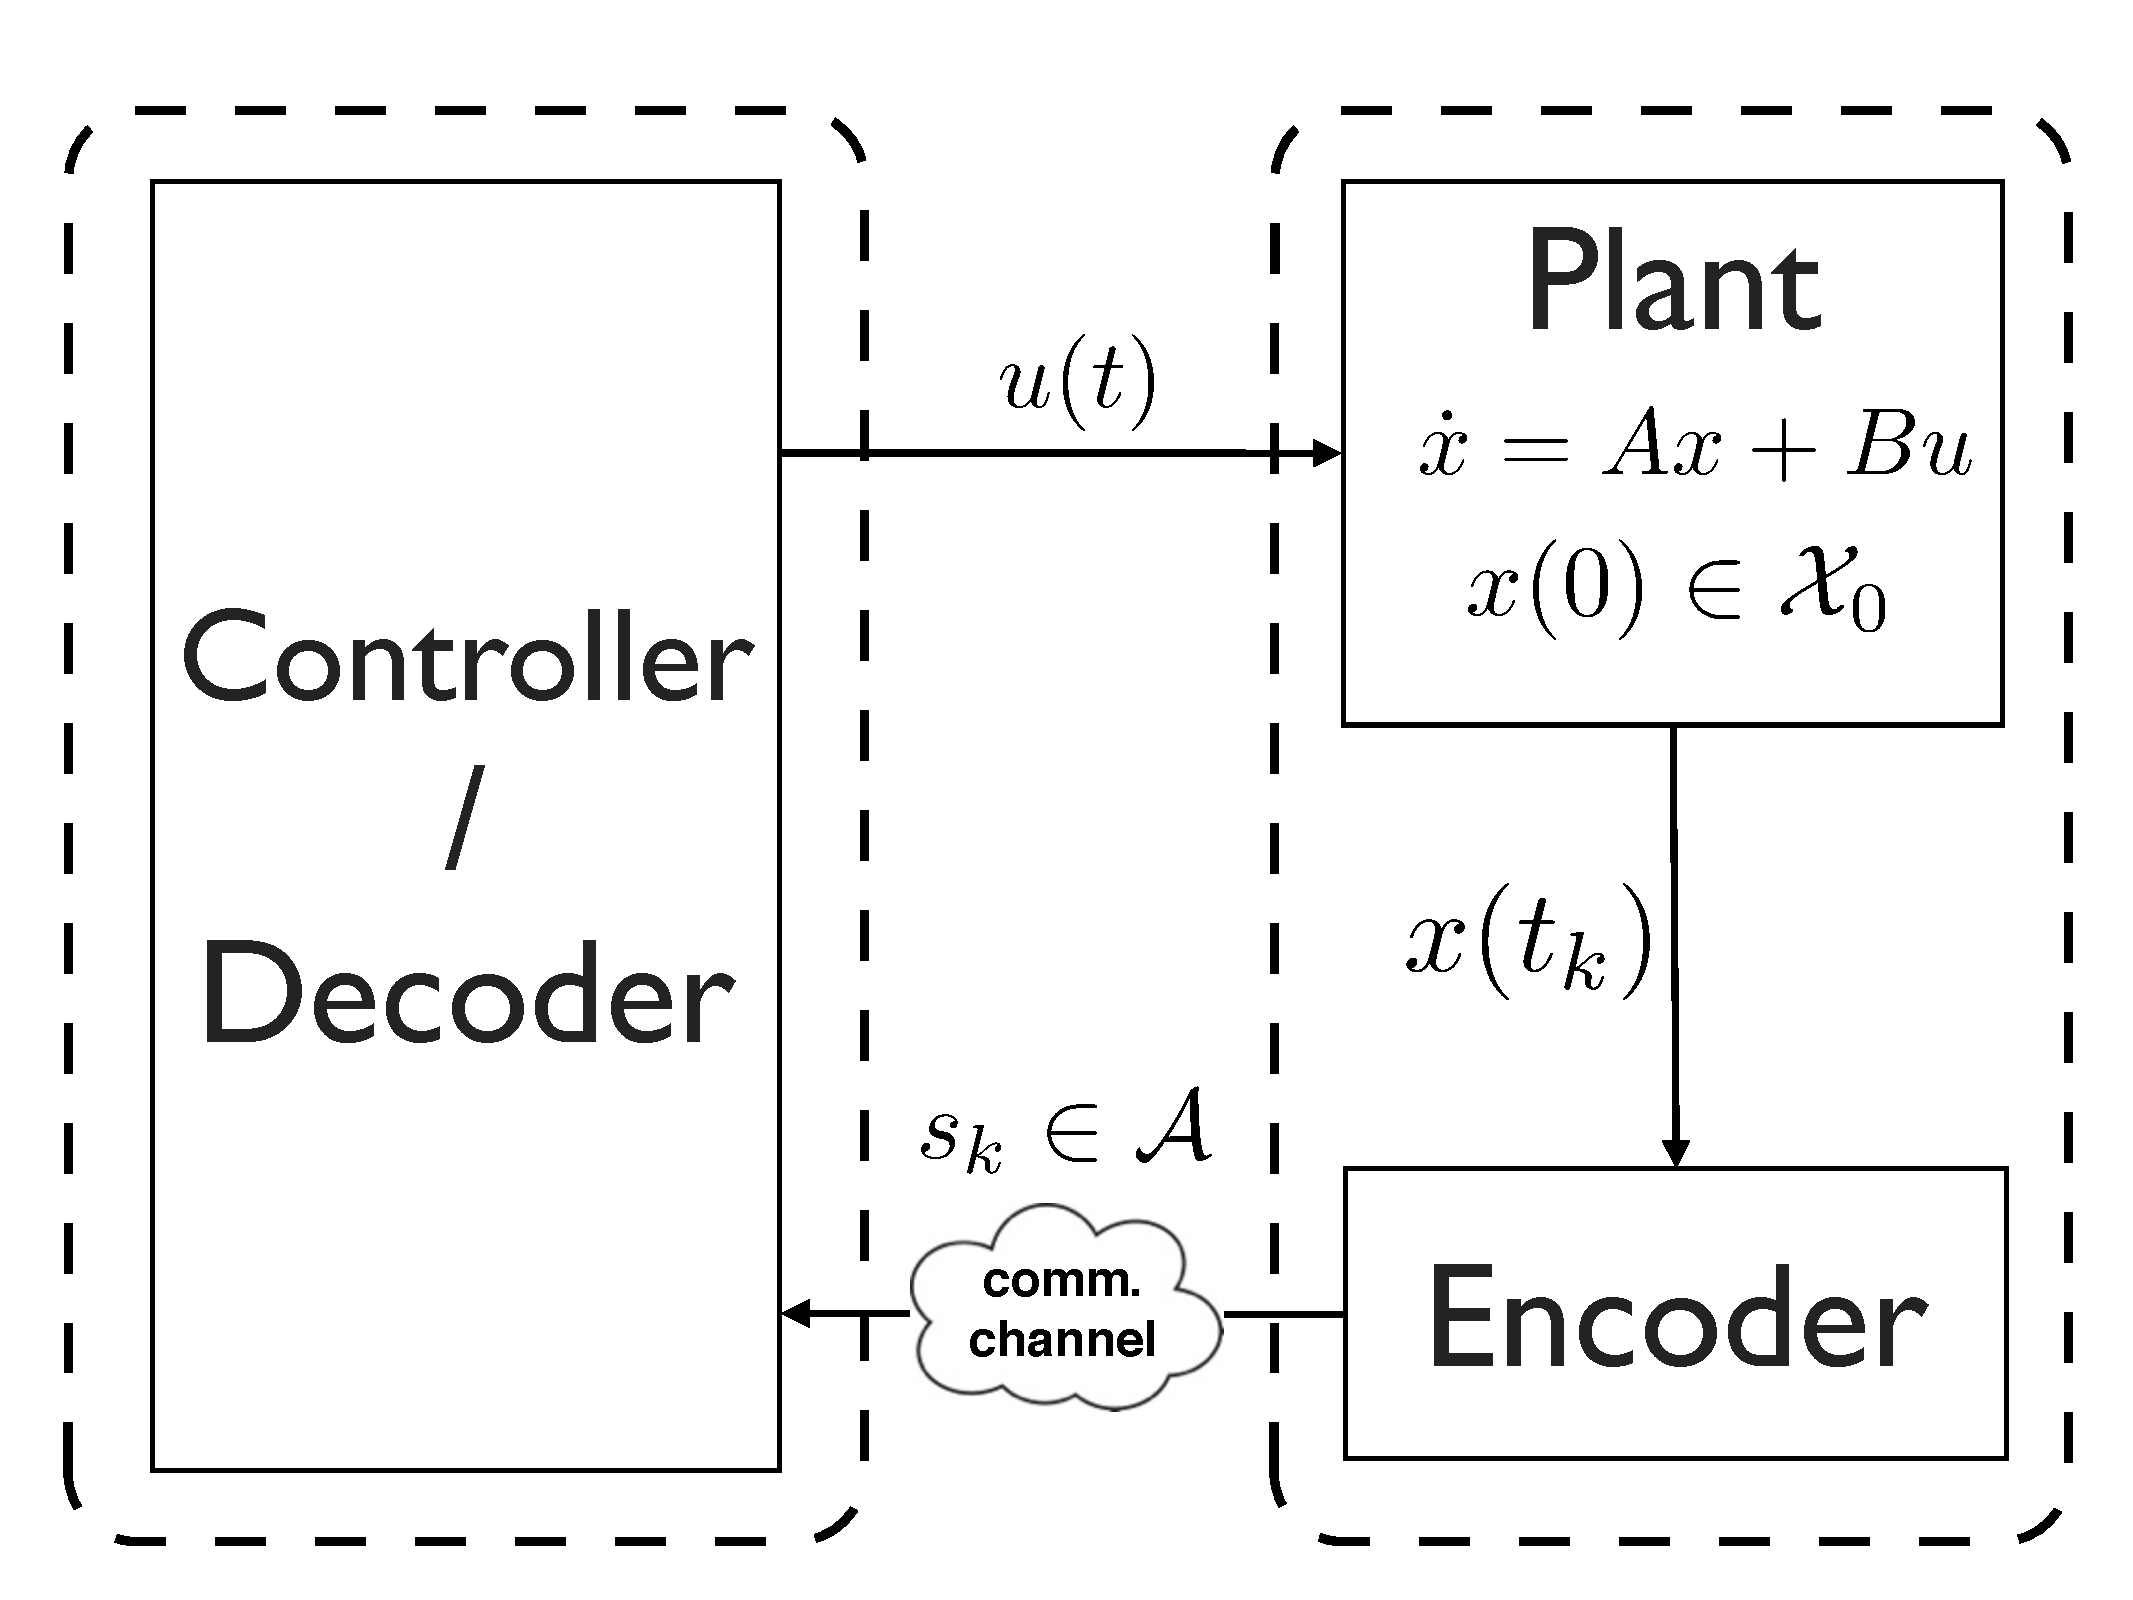
\includegraphics[angle=0,totalheight=.25\textheight]{figures/block-diagram}
  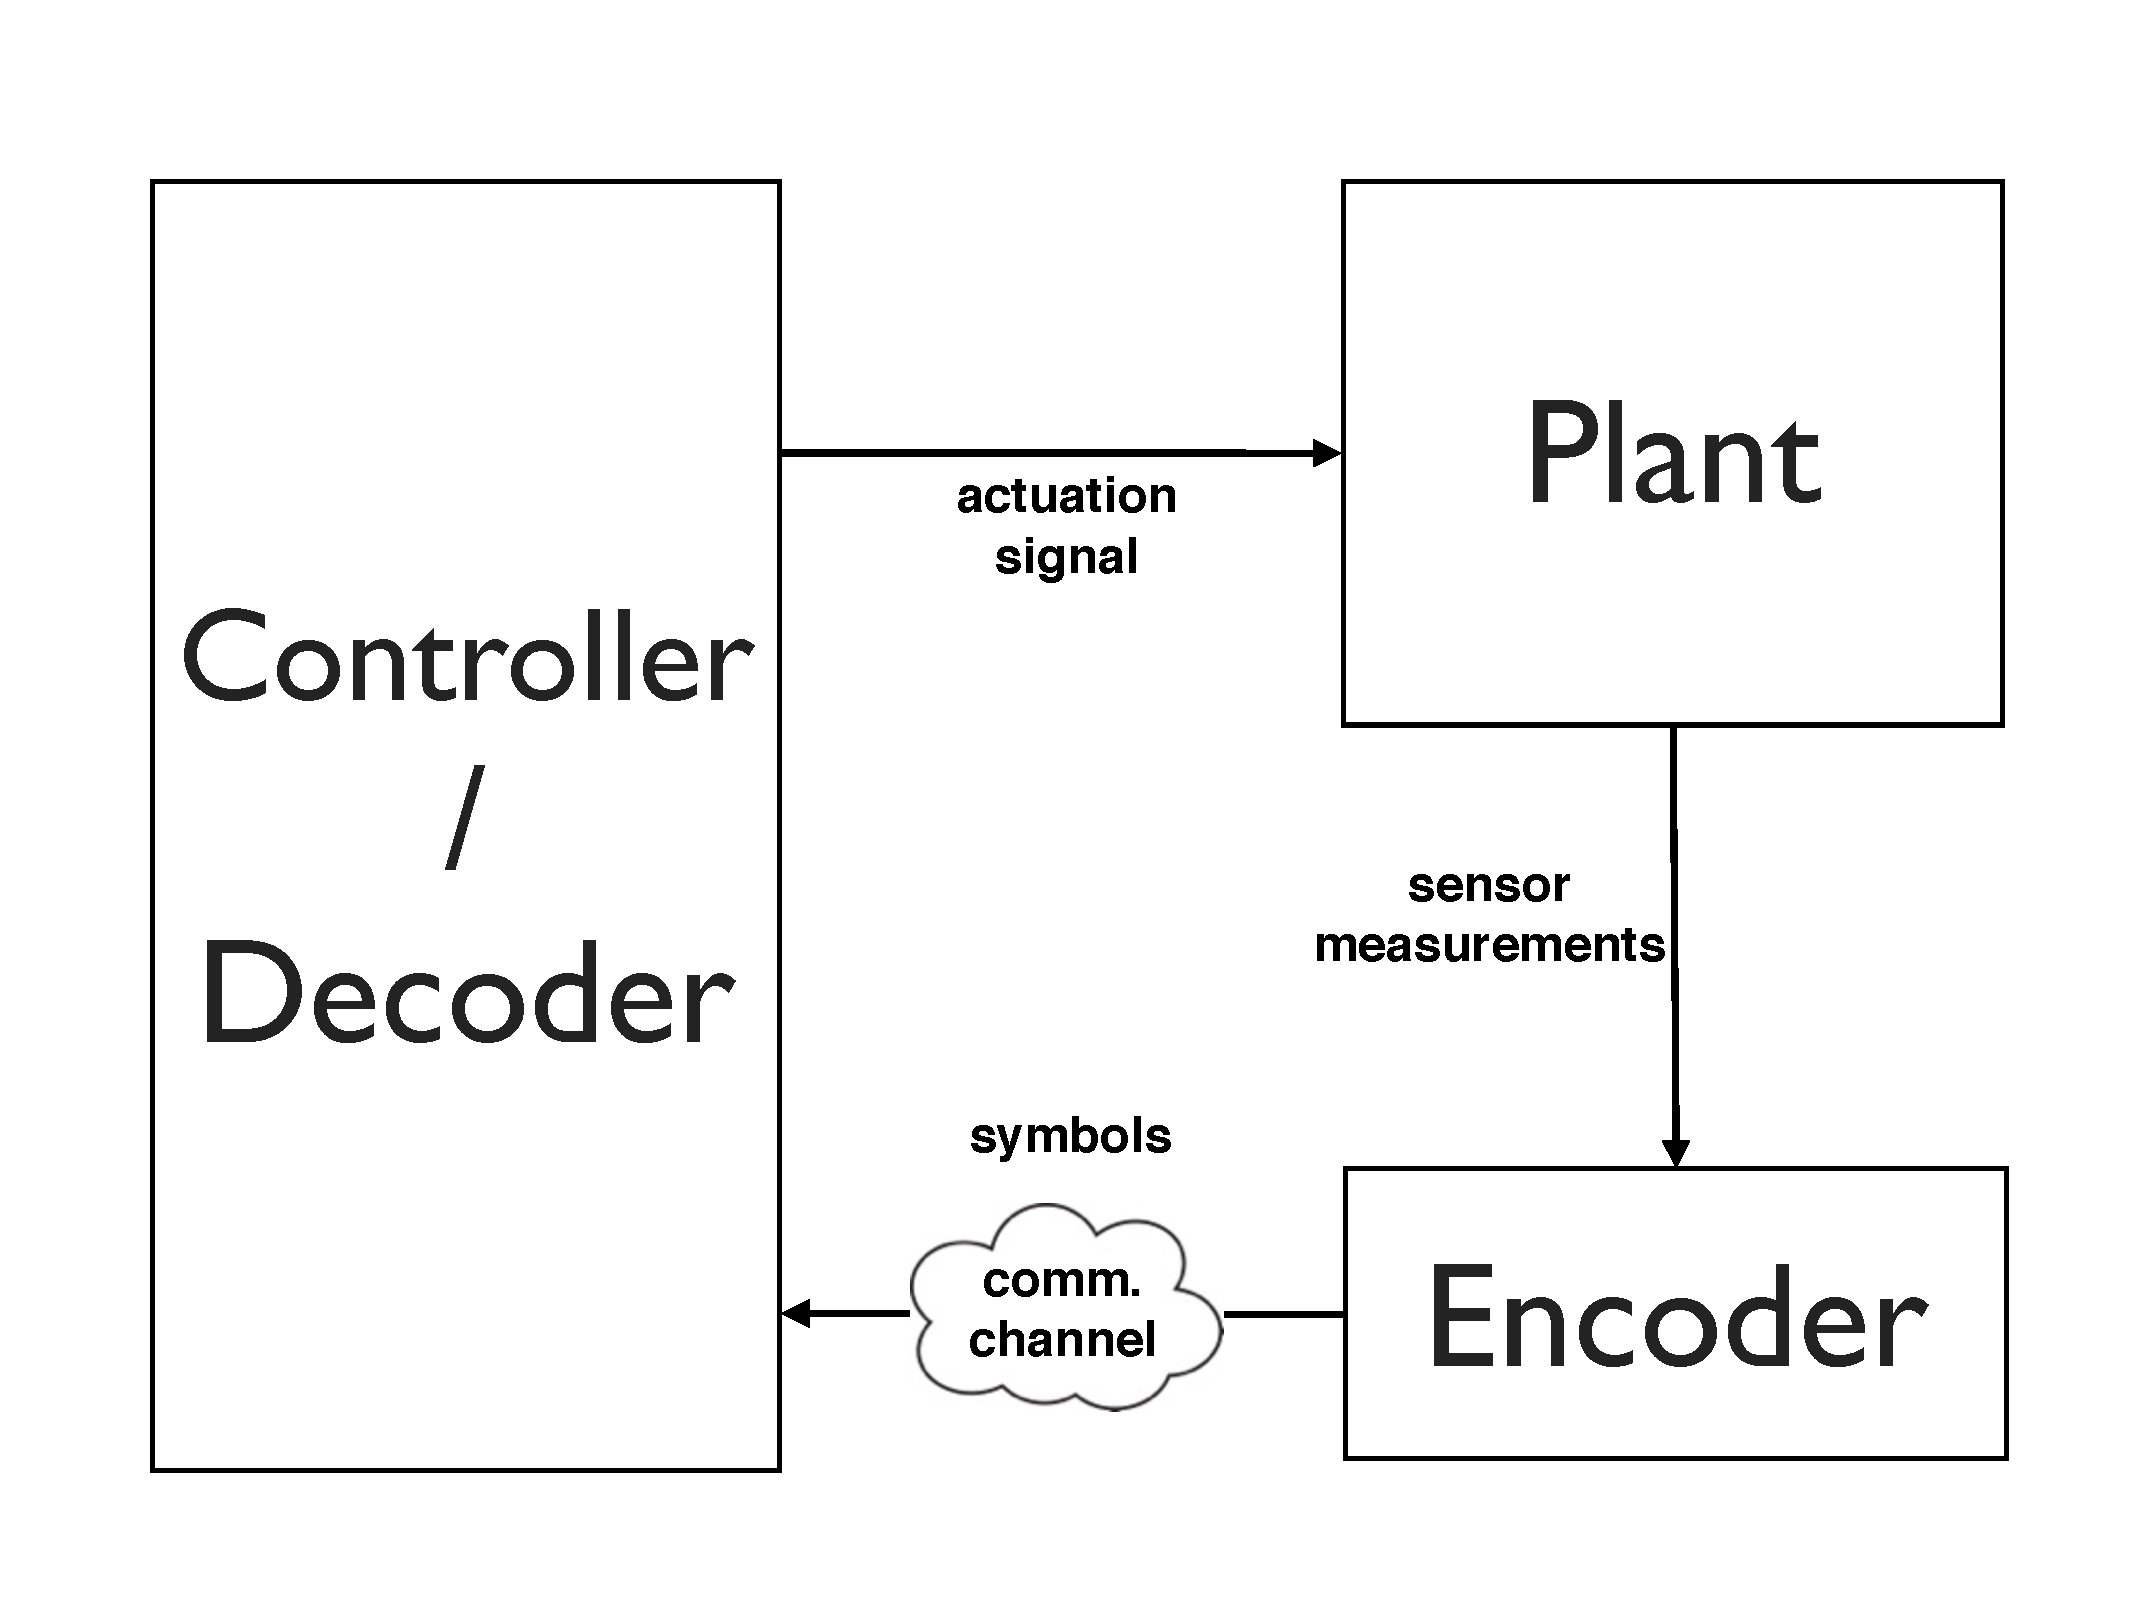
\includegraphics[angle=0,width=\figwidth]{figures/block_diagram_intro}
  \caption{The limited-communication control setup. At sampling times, the encoder measures the process state and selects
      symbols from a finite alphabet to send to the
      decoder/controller. The decoder/controller constructs the actuation
      signal for the plant.}
  \label{fig:block_diagram2}
\end{figure}

\subsection*{Prior work}

Variants of the limited-communication environment in Figure~\ref{fig:block_diagram2} were also considered in \cite{BrockettLiberzon2000,HespanhaOrtegaVasudevanAug02,NairEvans2000,TatikondaMitter2004,NairEvans2003,MatveevSavkin2005} and many other works. 

...


\subsection*{Contributions}

A starting point for the present work is the observation that an encoder can
effectively save communication resources by occasionally not
transmitting information --- the absence of an explicitly transmitted
symbol nevertheless conveys information. We formulate a framework to
capture this by supposing that each symbol's transmission costs one
unit of communication resources, except for one special free symbol that
represents the absence of a transmission.

...

\section*{\nameref{sxn:event-driven-encoders} (Chapter~\ref{sxn:event-driven-encoders})}

In Chapter~\ref{sxn:event-driven-encoders}, we use the framework from Chapter~\ref{chap:mineng} to analyze a family of event-based controllers.

...


\subsection*{Prior work}

Recent results in event-based
control
\cite{AstromBernhardsson2002,Astrom2007,Lunze2010211,TabuadaSep2007}
indicate that an encoder can conserve communication resources by
transmitting only on a ``need-to-know'' basis. 

...


\subsection*{Contributions}

In contrast to the optimal encoders introduced in Chapter~\ref{chap:mineng},
the proposed event-based encoders are easy to implement but not
optimal. However, they are only slightly sub-optimal. Specifically, ...


\section*{\nameref{chap:preemption} (Chapter~\ref{chap:preemption})}

The previous chapters indicate that networked control systems can benefit from precise timing by embedding information in the timing of messages. In Chapter~\ref{chap:preemption}, we turn our attention away from networked control systems and explore how precise timing can benefit a controller running (locally) on a non-real-time operating system. 

...


\subsection*{Background and prior work}

A program may execute nondeterministically for several reasons.

...



\subsection*{Contributions}

The specific contribution of this chapter is a controller architecture that
enables a controller to run on a non-real-time OS like Linux, yet
maintain precise timing of the sensing and actuation despite OS
preemption. This is achieved by performing the sensing and actuation
on a dedicated ``bare metal'' microcontroller that in essence serves
as a \rtio{}; we refer to this as the ``Real-Time Unit'' (\RTU{}). 


...




